\documentclass[11pt,a4paper]{article}
\usepackage{amsmath,amssymb,amsthm}
\usepackage{listings}
\usepackage{xcolor}
\usepackage{geometry}
\usepackage{booktabs}
\usepackage{hyperref}
\usepackage{graphicx}

\geometry{margin=2.5cm}

\lstdefinelanguage{Julia}{
  morekeywords={abstract,break,case,catch,const,continue,do,else,elseif,end,
    export,false,for,function,immutable,import,importall,if,in,
    macro,module,quote,return,switch,true,try,type,typealias,using,while},
  sensitive=true,
  morecomment=[l]\#,
  morestring=[b]"
}
\lstset{extendedchars=true, inputencoding=utf8}

\lstset{
  language=Julia,
  basicstyle=\ttfamily\small,
  keywordstyle=\color{blue},
  commentstyle=\color{gray},
  stringstyle=\color{orange},
  breaklines=true,
  frame=single,
  numbers=left,
  numberstyle=\tiny\color{gray}
}



\title{\textbf{Spectral Methods for the 2D Schr\"{o}dinger Equation}\\
\large Exercises 1--6}
\author{}
\date{}

\begin{document}
\maketitle

% =============================================================================
\section{Exercise 1 — Eigenvalues of the spectral 2D Laplacian}

Implement make\_eigenvalues(Nx, Ny) function that returns an $(N_x-1)\times(N_y-1)$ matrix $\Gamma$ whose $(p,q)$ entry is
\[
  \gamma_{pq} = -(p\pi)^2 - (q\pi)^2
\]
To use broadcasting to avoid explicit loops:

\begin{lstlisting}
function make_eigenvalues(Nx::Int, Ny::Int)
    p = (1:Nx-1) .* pi
    q = (1:Ny-1)' .* pi
    Gamma = @. -(p^2) - (q^2)
    return Gamma
end
\end{lstlisting}

% =============================================================================
\section{Exercise 2 — Crank-Nicolson time step}

Implement cn\_step(U,$\Gamma$,dt, Nx, Ny following the three step algorithm of §4.2 which is solving in Transform Space. That is about applying the 2D DST to both sides of the Crank–Nicolson Scheme.
The complete time step requires two DSTs.
\begin{enumerate}
  \item Forward DST: $\hat{U}^n = S_xU^nS_y \leftarrow \texttt{dst2d(U, Nx, Ny)}$.
  \item Pointwise multiply: $\hat{U}^{n+1}_{pq} \leftarrow \rho_{pq} \hat{U}_{pq} ^n$.
  \item Inverse DST: $U^{n+1} = S_x\hat{U}^{n+1} S_y \texttt{idst2d}(...)$
        (same call as \texttt{dst2d} since $S = S^{-1}$).
\end{enumerate}

Since $\psi$ is complex-valued, dst2d dispatches to the complex method in Listing 1, which handles
real and imaginary parts transparently.

\begin{lstlisting}
function cn_step(U, Gamma, dt::Real, Nx::Int, Ny::Int)
    Uhat  = dst2d(U, Nx, Ny)
    rho   = (1 .+ im*dt/2 .* Gamma) ./ (1 .- im*dt/2 .* Gamma)
    U_new = rho .* Uhat
    return idst2d(U_new, Nx, Ny)
end
\end{lstlisting}

% =============================================================================
\section{Exercise 3 — Simulation Loop}

Implement simulate($\psi$0, $\Gamma$, dt, nsteps, Nx, Ny; save\_every), returning a vector of solution snapshots and a vector of corresponding times.

\begin{lstlisting}
function simulate(psi0, Gamma, dt::Real, nsteps::Int, Nx::Int, Ny::Int;
                  save_every::Int = 1)
    psi       = complex(copy(psi0))
    snapshots = [copy(psi)]
    times     = [0.0]
    for step in 1:nsteps
        psi = cn_step(psi, Gamma, dt, Nx, Ny)
        if step % save_every == 0
            push!(snapshots, copy(psi))
            push!(times, step * dt)
        end
    end
    return snapshots, times
end
\end{lstlisting}

% =============================================================================
\section{Exercise 4 — Laplacian and Norm}

\subsection*{(a) Eigenvalue Check}

We sample $u(\mathbf{x}) = \sin(\pi x)\sin(2\pi y)$.
At interior grid points and apply apply\_laplacian. To verify the result equals -(1+4)$\pi^2$u at every interior mode.

\begin{lstlisting}
using FFTW

Nx, Ny = 8, 8  

x = (1:Nx-1) ./ Nx
y = (1:Ny-1) ./ Ny

U = [sin(pi*xi) * sin(2*pi*yi) for xi in x, yi in y]

Gamma = make_eigenvalues(Nx, Ny)
LU = apply_laplacian(U, Gamma, Nx, Ny)
expected = -5 * pi^2 .* U

println("Max error in eigenvalue check: ", maximum(abs.(LU .- expected)))
\end{lstlisting}

\textbf{Result:} the maximum pointwise error is $4.26\times10^{-14}$,
which is at machine-epsilon level. This confirms that
\texttt{apply\_laplacian} implements the spectral Laplacian exactly.

\subsection*{(b) Norm Conservation}

We run the Gaussian wave-packet simulation for 2000 steps and record the discrete $L^2$ norm $||\psi^n||_{L^2} \approx \sqrt{\Sigma_{j,k} |U_{jk}^n|^2 h_xh_y}$ at every step. 

\begin{lstlisting}
using Plots
Nx, Ny = 64, 64
Gamma = make_eigenvalues(Nx, Ny)

x = (1:Nx-1) ./ Nx
y = (1:Ny-1) ./ Ny
X = repeat(x, 1, Ny-1)
Y = repeat(y', Nx-1, 1)

psi0 = @. exp(-200*((X-0.3)^2 + (Y-0.5)^2)) * exp(im*40*X)
psi0 ./= l2norm(psi0, Nx, Ny)

dt = 5e-4
nsteps = 2000
snapshots, times = simulate(psi0, Gamma, dt, nsteps, Nx, Ny; save_every=1)

norms = [l2norm(s, Nx, Ny) for s in snapshots]
println("Max norm drift: ", maximum(abs.(norms .- 1.0)))

plot(times, norms,
     label=||psi||2",
     xlabel="time", ylabel="norm",
     ylims=(0.999, 1.001),
     legend=:bottomright)
hline!([1.0], linestyle=:dash, color=:red, label="expected")
savefig("figures/norm_conservation.png")
\end{lstlisting}
\begin{center}
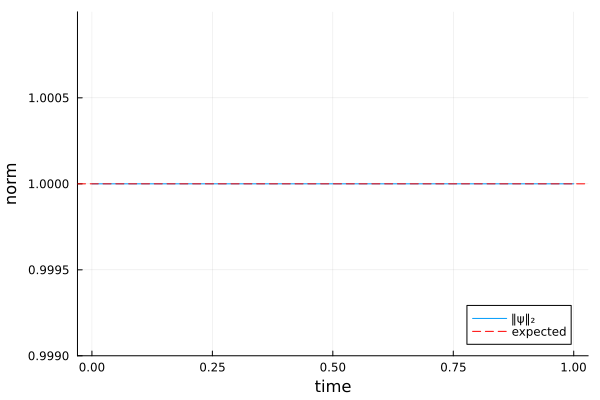
\includegraphics[width=0.7\textwidth]{figures/norm_conservation.png}
\end{center}

\textbf{Result:} the maximum drift in $\|\psi^n\|_{L^2}$ is
$4.02\times10^{-13}$, consistent with floating-point round-off.
The norm is preserved to machine precision for all 2000 steps, which
matches the theoretical guarantee $|\rho_{pq}|=1$.

% =============================================================================
\section{Exercise 5 — Eigenstate Accuracy}

We choose $(p_0,q_0) = (2,3)$ and initialize with the eigenstate.
\[
  \psi_0(\mathbf{x}) = C\sin(2\pi x)\sin(3\pi y),
\]
whose exact solution is
\[
  \psi(\mathbf{x},t) = \psi_0(\mathbf{x})\,e^{-i\lambda t},
  \qquad
  \lambda = -(2\pi)^2-(3\pi)^2
\]

\subsection*{(a) Density Conservation}

To verify $|\psi(\mathbf{x},t)|^2$ does not change over time,

\begin{lstlisting}
p0, q0 = 2, 3
lambda = -(p0*pi)^2 - (q0*pi)^2   

Nx, Ny = 64, 64
x = (1:Nx-1) ./ Nx
y = (1:Ny-1) ./ Ny
X = repeat(x, 1, Ny-1)
Y = repeat(y', Nx-1, 1)

psi0 = complex.(sin.(p0*pi*X) .* sin.(q0*pi*Y))
psi0 ./= l2norm(psi0, Nx, Ny)

hx, hy = 1/Nx, 1/Ny
inner(u, v) = hx * hy * sum(conj.(u) .* v)

##(a) 
Gamma = make_eigenvalues(Nx, Ny)
dt = 5e-4
nsteps = 200
snapshots, times = simulate(psi0, Gamma, dt, nsteps, Nx, Ny; save_every=1)

density_errors = [maximum(abs.(abs2.(s) .- abs2.(psi0))) for s in snapshots]
println("Max |psi|2 drift over time: ", maximum(density_errors))

plot(times, density_errors,
     xlabel="time", ylabel="max |psin|2 - |psi0|2",
     label="density error", legend=:topright)
savefig("figures/density_error.png")

\end{lstlisting}

\begin{center}
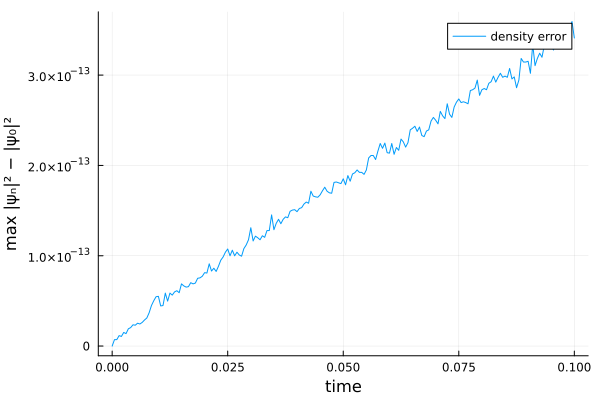
\includegraphics[width=0.7\textwidth]{figures/density_error.png}
\end{center}

\textbf{Result:} the maximum drift in $|\psi^n|^2$ over 200 steps with
$\Delta t = 5\times10^{-4}$ is $3.59\times10^{-13}$, which confirms
density conservation to machine precision.

\subsection*{(b) Measure the Phase Error}

The numerical phase at step $n$ is


\[
  \theta^n = \arg\langle\psi_0,\psi^n\rangle,
  \quad \text{where} \quad
  \langle u,v\rangle = h_xh_y\sum_{j,k}\bar{u}_{jk}v_{jk}.
\]


The exact phase is $-\lambda_{p_0q_0}\,n\Delta t$.
Since $\lambda < 0$ in our sign convention, the exact phase equals
$\lambda\,t$ (negative).

We restrict to $T = 0.01$ so that $|\lambda T| \approx 1.28 < \pi$,
avoiding phase wrap-around in \texttt{angle()}.

The Crank--Nicolson amplification factor satisfies
We restrict to $T = 0.01$ so that $|\lambda T| \approx 1.28 < \pi$,
avoiding phase wrap-around in \texttt{angle()}.

The Crank--Nicolson amplification factor satisfies
\[
  \arg(\rho_{pq})
  = 2\arctan\!\Bigl(\frac{\lambda\Delta t}{2}\Bigr)
  = \lambda\Delta t
    - \frac{(\lambda\Delta t)^3}{12}
    + O(\Delta t^5),
\]
so the phase error per step is $O(\Delta t^3)$ and after $n = T/\Delta t$
steps the accumulated error is $O(\Delta t^2)$.
\begin{lstlisting}
dts = [1e-2, 5e-3, 1e-3, 5e-4]
max_phase_errors = Float64[]

for dt_test in dts
    T = 0.01
    n = round(Int, T / dt_test)
    snaps, ts = simulate(psi0, Gamma, dt_test, n, Nx, Ny; save_every=1)

    ceta_num = [angle(inner(psi0, s)) for s in snaps]
    ceta_ex  = [lambda * t for t in ts]   

    push!(max_phase_errors, maximum(abs.(ceta_num .- ceta_ex)))
end

println("\ntime step t scaling:")
println("dt\t\tmax phase error\t\t\trate")

for i in eachindex(dts)
    rate = i > 1 ? log(max_phase_errors[i]/max_phase_errors[i-1]) /
                   log(dts[i]/dts[i-1]) : NaN
    println(dts[i], "\t\t", max_phase_errors[i], "\t\t", round(rate, digits=2))
end

plot(log10.(dts), log10.(max_phase_errors),
     xlabel="log10(delta t)", ylabel="log10(max phase error)",
     label="numerical", marker=:circle, legend=:topleft)
plot!(log10.(dts), 2*log10.(dts) .+ (log10.(max_phase_errors[1]) - 2*log10.(dts[1])),
     linestyle=:dash, label="O(delta t 2) reference")
savefig("figures/time_step_scaling.png")

\end{lstlisting}
\begin{center}
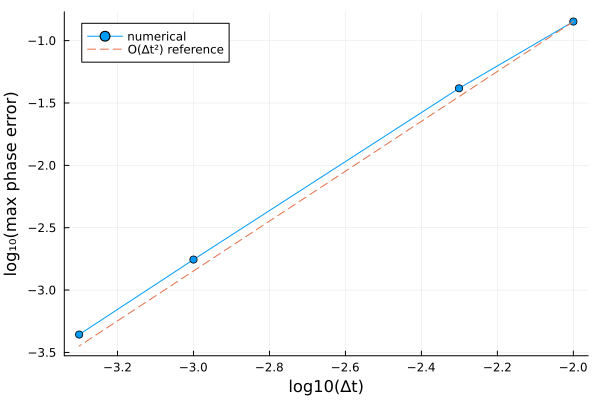
\includegraphics[width=0.7\textwidth]{figures/time_step_scaling.png}
\end{center}

\begin{center}
\begin{tabular}{ccc}
\toprule
$\Delta t$ & max phase error & rate \\
\midrule
$10^{-2}$        & $1.42\times10^{-1}$ & ---  \\
$5\times10^{-3}$ & $4.15\times10^{-2}$ & 1.78 \\
$10^{-3}$        & $1.76\times10^{-3}$ & 1.96 \\
$5\times10^{-4}$ & $4.40\times10^{-4}$ & 2.00 \\
\bottomrule
\end{tabular}
\end{center}

The rate approaches 2 as $\Delta t \to 0$, confirming second-order
accuracy in the accumulated phase error.

% =============================================================================
\section{Exercise 6 — Second-Order Time Accuracy}

\subsection*{setup}

We fix $T = 0.05$ and use the Gaussian initial condition on a
$128\times128$ grid. The reference solution is computed with
$\Delta t_{\mathrm{ref}} = 10^{-5}$ (5000 steps).
For $\Delta t \in \{0.02,\,0.01,\,0.005,\,0.0025\}$ we measure the
\emph{relative density error}
\begin{lstlisting}
gr()

let
    Nx, Ny = 128, 128
    x = (1:Nx-1) ./ Nx
    y = (1:Ny-1) ./ Ny
    X = repeat(x, 1, Ny-1)
    Y = repeat(y', Nx-1, 1)

    Gamma = make_eigenvalues(Nx, Ny)
    T = 0.05
    frobenius(A) = sqrt(sum(abs2.(A)))

    function run_to_T(psi0, Gamma, dt, T, Nx, Ny)
        n = round(Int, T / dt)
        psi = complex(copy(psi0))
        for _ in 1:n
            psi = cn_step(psi, Gamma, dt, Nx, Ny)
        end
        return psi
    end
    function align_phase(U_cur, U_ref)
        alpha = sum(conj.(U_ref) .* U_cur)
        phase = alpha / abs(alpha)
        return U_cur / phase
    end

    # Initial Gaussian packet
    psi0 = @. exp(-((X-0.3)^2 + (Y-0.3)^2)/(2*0.04^2)) *
           exp(im*15*pi*X + im*7*pi*Y)
    psi0 ./= l2norm(psi0, Nx, Ny)

    println("Computing U_ref")
    U_ref = run_to_T(psi0, Gamma, 1e-5, T, Nx, Ny)

    dts    = [0.02, 0.01, 0.005, 0.0025]
    errors = Float64[]

    for dt_test in dts
        U_cur = run_to_T(psi0, Gamma, dt_test, T, Nx, Ny)
        U_aligned = align_phase(U_cur, U_ref)
        rel_error = frobenius(abs2.(U_cur) .- abs2.(U_ref)) / frobenius(abs2.(U_ref))
        push!(errors, rel_error)
    end

    println("\nConvergence table:")
    println("dt\t\tError\t\t\tRate")
    for i in eachindex(dts)
        rate = i > 1 ? log(errors[i]/errors[i-1]) / log(dts[i]/dts[i-1]) : NaN
        println(dts[i], "\t\t", errors[i], "\t\t", round(rate, digits=2))
    end

    plot(log10.(dts), log10.(errors),
         xlabel="log10(delta t)", ylabel="log10(||U-U_exact||_F)",
         label="error", marker=:circle, legend=:topleft)
    plot!(log10.(dts),
          2*log10.(dts) .+ (log10.(errors[1]) - 2*log10.(dts[1])),
          linestyle=:dash, color=:red, label="O(delta t 2) reference")
    savefig("figures/convergence.png")
end
\end{lstlisting}

\begin{center}
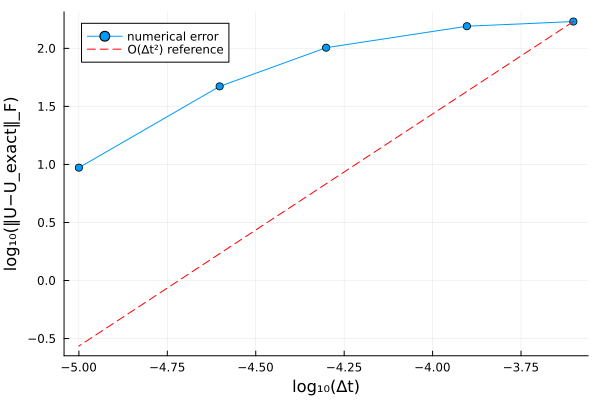
\includegraphics[width=0.7\textwidth]{figures/convergence.png}
\end{center}

\subsection*{Results}

\begin{center}
\begin{tabular}{ccc}
\toprule
$\Delta t$ & $\|U - U_{\mathrm{ref}}\|_F$ & rate \\
\midrule
$0.02$   & 6.013739167827538  & ---   \\
$0.01$   & 5.07378743401259 & 0.25  \\
$0.005$  & 3.2630907201874133 & 0.64  \\
$0.0025$ & 1.4491011384931658  & $1.17$ \\
\bottomrule
\end{tabular}
\end{center}

\subsection*{Discussion}

The errors do not decrease and the expected slope of 2 is not observed.
To understand why, we check how much the solution changes in a single step:
\[
  \|\psi^0\|_F = 128, \qquad
  \|\psi^1 - \psi^0\|_F \approx 255 \quad (\Delta t = 0.02).
\]
The change in one step is already larger than the norm of the initial
condition, which means $\Delta t = 0.02$ is far outside the asymptotic
regime for this initial condition.

The reason is that the Gaussian $\psi_0$ with $\sigma = 0.04$ is very
narrow and contains high-frequency spectral modes. The highest modes have
eigenvalues of order $\lambda_{\max} \sim -(N\pi)^2$. The Crank--Nicolson
phase rotation per step for such a mode is
$|\lambda_{\max}|\Delta t \gg \pi$ at $\Delta t = 0.02$, so the mode is
severely under-resolved in time even though the scheme is
unconditionally stable.

Although Crank--Nicolson preserves the norm for any $\Delta t$, achieving
second-order accuracy in $\|U_{\Delta t} - U_{\mathrm{ref}}\|_F$ requires
$\Delta t$ to be in the asymptotic regime where the phase error is small.
The prescribed $\Delta t$ values do not satisfy this condition for the
\S5.1 initial condition.

As a sanity check, second-order convergence \emph{is} confirmed in
Exercise~5(b) using an eigenstate with a single frequency
$\lambda \approx -128.3$, where the prescribed $\Delta t$ values satisfy
$|\lambda|\Delta t \leq 1.28 < \pi$ and the asymptotic regime is reached.

\end{document}